% 
% 
%			6: Experiment: MapReduce
\chapter{Experiment: MapReduce}
\label{chap:map-reduce}

Although the full dataset is processed pretty quickly I would like to implement the map reduce algorithm in order to make the entire implementation faster.
No external libraries will be used, the solution will be based on python multiprocessing.
Experiment: 
Analysing the data processing steps, I have come to the conclusion that the slowest part is selecting baskets with frequent items. My MapReduce implemention will consist of:

\begin{itemize}
	\item Map step: check if a basket contains any of the frequent items
	\item Reduce step: aggregate the results
\end{itemize}

The analysis of time required for selecting rows with frequent items shows that the custom MapReduce implementation performs faster than pandas filtering at small dataset sizes (up to hundreds of thousands of rows). The pandas selection performs almost at a constant time, while custom implementation needs more time as dataset becomes larger.
This fact may highlight the drawbacks of custom implementation, persumably, in the reduce algorithm.

\begin{figure}[h]
	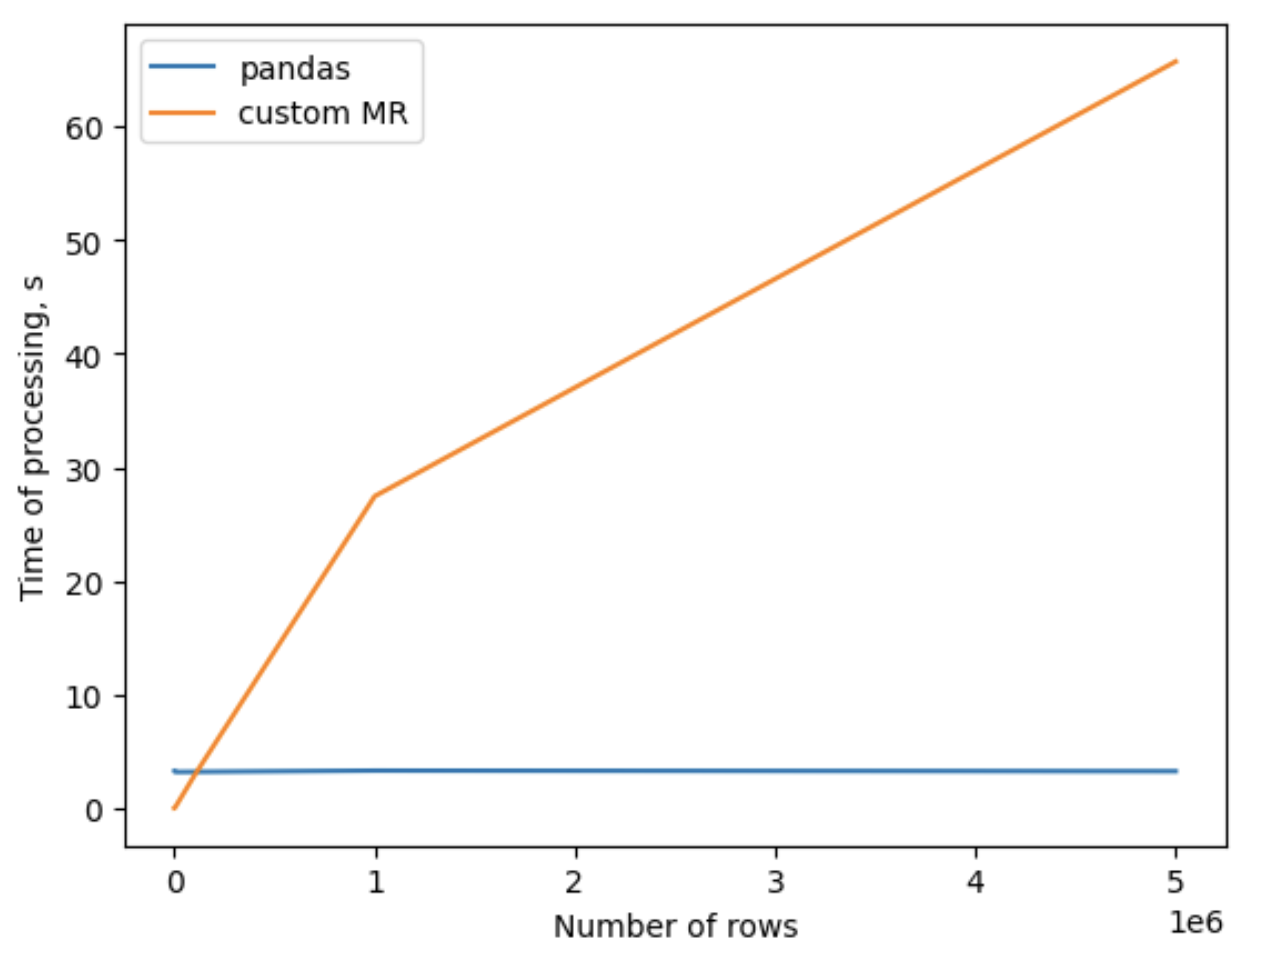
\includegraphics[width=12cm]{images/6-map_reduce_timings}
\centering
\end{figure}

